\documentclass[a4paper, 11pt,table]{article}

\usepackage[utf8]{inputenc}
\usepackage[T1]{fontenc}
\usepackage[toc,page]{appendix}
\usepackage{varioref}
\usepackage{hyperref}
\usepackage[nameinlink]{cleveref}
\usepackage{nameref}
\usepackage{parskip}
\usepackage{multicol}%multi column bib
\usepackage[sectionbib, tocbib, numberedbib, bibnewpage]{apacite}%Citations
\usepackage{tikz}
\usepackage{pdflscape}
\usepackage{tabu}
\usepackage{pgfplots}

\bibliographystyle{apacite}

\author{Steven Lowes}
\title{Software Methodologies AI Search}
\date{\today{}}

\newcommand{\smartref}[1]{%
	\hyperref[#1]{\cref{#1}, ``\nameref{#1}", \vpageref{#1}}%
}

\begin{document}

	\section{Algorithm A: Simulated Annealing}
	
	\subsection{Results}
	\label{useCase:annealResults}
	\begin{center}
		\rowcolors{0}{gray!25}{white}
		\begin{tabu}{|c c c|}
			\textbf{Nodes} & \textbf{Tour Length} & \textbf{Runtime (s)}\\
			12 & 56.0 & 0.11s \\
			17 & 1,514 & 2.42s\\
			21 & 2,716 & 2.46s\\
			26 & 1,487 & 9.08s\\
			42 & 1,217 & 9.64s\\
			48 & 14,846 & 14.66s\\
			58 & 26,740 & 13.95s\\
			175 & 21,613 & 2m10s\\
			180 & 2,720 & 2m16s\\
			535 & 50,191 & 13m23s\\
		\end{tabu}
	\end{center}

	\begin{center}
		\rowcolors{0}{gray!25}{white}
		\begin{tabu}{|c c c|}
			\textbf{Iterations (m)} & \textbf{Tour Length} & \textbf{Runtime (s)}\\
			6.6 & 55,111 & 1.99s\\
			33 & 53,643 & 8.40s\\
			99 & 52,678 & 23.2s\\
			331 & 50,928 & 1m15s\\
			893 & 50,301 & 3m25s\\
			2,648 & 50,191 & 13m23s \\
		\end{tabu}
	\end{center}

	\begin{center}
		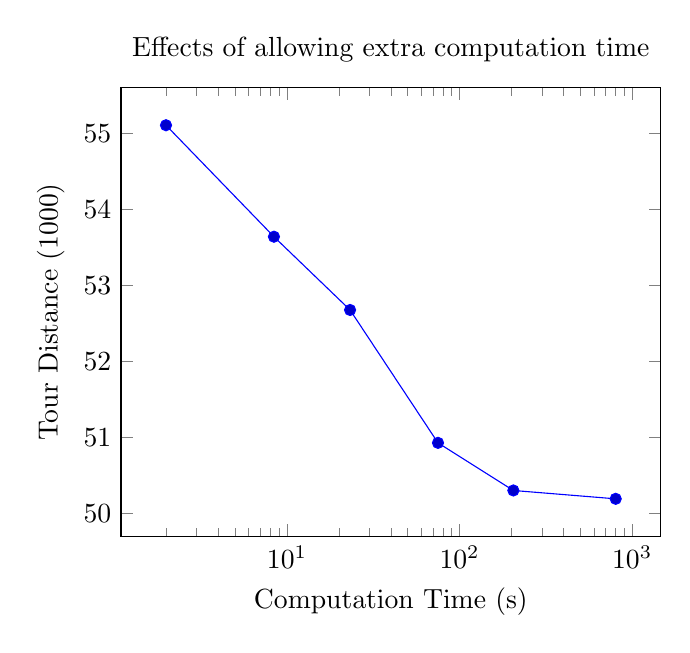
\begin{tikzpicture}
			\begin{axis}[
			title = Effects of allowing extra computation time,
			xlabel = {Computation Time (s)},
			ylabel = {Tour Distance (1000)},
			xmode=log,
			]
				\addplot coordinates {
				(1.99,55.111)
				(8.40,53.643)
				(23.2,52.678)
				(75,50.928)
				(205,50.301)
				(803,50.191)
			};
			\end{axis}
		\end{tikzpicture}
	\end{center}

\subsection{Description}
Simulated annealing is similar to a hill climbing algorithm, except it will occasionally move down the hill. The chance of doing so decreases as the algorithm nears completion.

Start Temp

End Temp

Multithreading

Cooling Rate
	
	\section{Algorithm B: Ant Colony Optimisation}
	
		\subsection{Results}
	\label{useCase:antResults}
	\begin{center}
		\rowcolors{0}{gray!25}{white}
		\begin{tabu}{|c c c|}
			\textbf{Nodes} & \textbf{Tour Length} & \textbf{Runtime (s)}\\
			12 & 56.0 & 0.60s \\
			17 & 1,444 & 1.02s\\
			21 & 2,549 & 1.28s\\
			26 & 1,575 & 2.98s\\
			42 & 1,322 & 6.27s\\
			48 & 12,702 & 15.72s\\
			58 & 25,855 & 19.10s\\
			175 &  21,770 & 2m25s\\
			180 & 1,950 & 3.42s\\
			535 & 53,409 & 9.4ss\\
			535 & 50,762 & 1m4s\\
			535 & 50,124 & 11m16s\\
		\end{tabu}
	\end{center}

\subsection{Description}
Ant Colony Optimisation simulates a number of ants moving around the graph. At each junction the ant chooses an edge to travel down using a weighted random selection. The weights for each edge are based on the amount of `pheremones' on that edge and the edge's length. Shorter edges are more desirable, as are edges with more pheremones. After each iteration, all ants deposit pheremones on the paths they travelled down. Pheremones then evaporate, with the pheremones on each edge being multiplied by a constant factor.

Desirability
\begin{equation}
Desirability = Pheremones^{2}*Length^{-2}
\end{equation}

Elite Ant

Multithreading

Culling

Fast array
	\end{document}
